\section{Appendix C:  Additional Material}

\subsection{Derivation of the Law of Sines}

The Law of Sines shows a fundamental relationship between the interior angles of a triangle and the lengths of its sides.  For a triangle with sides of length $A$, $B$, and $C$, with opposing interior angles $a$, $b$, and $c$.\\

\begin{figure}[htb]
\center
\caption{A triangle.}
\label{fig:A triangle}
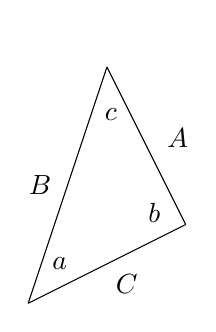
\begin{tikzpicture}[inner sep=0pt,minimum size=0mm]

\node () at (0,3.5) {};

\draw[] (0,0) -- (2,1);
\draw[] (2,1) -- (1,3);
\draw[] (1,3) -- (0,0);

\node () at (0.4,0.5){$a$};
\node () at (1.6,1.15) {$b$};
\node () at (1.05,2.4) {$c$};

\node () at (1.9,2.1){$A$};
\node () at (0.15,1.5) {$B$};
\node () at (1.25,0.25) {$C$};

\end{tikzpicture}
\end{figure} 

The Law of Sines states that:\\


\tab$\frac{A}{sin(a)} = \frac{B}{sin(b)} = \frac{C}{sin(c)}$\\

This can be derived readily for acute angles using the definition of sine.  Given a triangle, draw a line from one vertex perpendicular to the opposing side.  This line splits the triangle into two right triangles.  We assume this line has a length of $Y$.\\

\begin{figure}[htb]
\center
\caption{A triangle with acute angles.}
\label{fig:A triangle}
\begin{tikzpicture}[inner sep=0pt,minimum size=0mm]

\node () at (0,3.5) {};

\draw[] (0,0) -- (6,0);
\draw[] (6,0) -- (4,3);
\draw[] (4,3) -- (0,0);

\draw[] (4,3) -- (4,0);

\draw[] (4,0.25) -- (3.75,0.25) -- (3.75,0);


\node () at (0.75,0.25){$a$};
\node () at (5.5,0.25) {$b$};
\node () at (3.85,2.5) {$c$};

\node () at (5.5,1.5){$A$};
\node () at (1.4,1.5) {$B$};
\node () at (3,-0.5) {$C$};

\node () at (4.3,1) {$Y$};

\end{tikzpicture}
\end{figure}

Using the definition of sine, we can state:\\

\tab $sin(a) = \frac{Y}{B}$  and  $sin(b) = \frac{Y}{A}$\\

We can rearrange our definitions to be equal:\\

\tab $B sin(a) = Y$  and $A sin(b) = Y$ \\

\tab $\implies B sin(a) = A sin(b)$\\

\tab $\implies \frac{sin(a)}{A} = \frac{sin(b)}{B}$\\

A similar, derivation is possible when comparing an acute angle and an obtuse angle.  We still project a line of length $Y$ down at a right angle to its opposing side:\\

\begin{figure}[htb]
\center
\caption{A triangle with and obtuse angle.}
\label{fig:A triangle}
\begin{tikzpicture}[inner sep=0pt,minimum size=0mm]

\node () at (0,3.5) {};

\draw[] (0,0) -- (4,0);
\draw[] (4,0) -- (6,3);
\draw[] (6,3) -- (0,0);

\draw[] (6,3) -- (6,0);

\draw[dashed] (6,0) -- (4,0);

\draw[] (6,0.25) -- (5.75,0.25) -- (5.75,0);


\node () at (1.25,0.25){$a$};
\node () at (3.75,0.25) {$b$};
\node () at (5.1,2.25) {$c$};
\node () at (4.85,0.25) {$180-b$};

\node () at (5,1){$A$};
\node () at (1.4,1.5) {$B$};
\node () at (3,-0.5) {$C$};

\node () at (6.3,1.5) {$Y$};

\end{tikzpicture}
\end{figure}

Using the definition of sine, we can state:\\

\tab $sin(a) = \frac{Y}{B}$  and  $sin(180-b) = \frac{Y}{A}$\\

As well, from the sum of two angles, we can show that $sin(180-x) = sin(x)$:\\

\tab $sin(180-x) = sin(180)cos(x) - cos(180)sin(x)$\\

\tab $= (0)cos(x) - (-1)sin(x)$\\

\tab $= sin(x)$\\

Thus:\\

\tab $B sin(a) = Y$  and $A sin(b) = Y$ \\

\tab $\implies B sin(a) = A sin(b)$\\

\tab $\implies \frac{sin(a)}{A} = \frac{sin(b)}{B}$\\

When the angle $b$ is a right angle, we know that $Y = A$, thus:\\

\tab $sin(b) = 1 = \frac{A}{A}$ and $sin(a) = \frac{A}{B}$\\

\tab $\implies A sin(b) = A$ and $B sin(a) = A$\\

\tab $\implies A sin(b) = B sin(a)$\\

\tab $\implies \frac{sin(b)}{B} = \frac{sin(a)}{A}$\\

This can also be derived using the assumptions made for the the case of an obtuse angle, the result is the same either way.\\

From these three proofs, we can show equaltiy for any sets of sides and angles, thus:\\

\tab$\frac{A}{sin(a)} = \frac{B}{sin(b)} = \frac{C}{sin(c)}$\\


\clearpage
\subsection{Derivation of the Law of Cosines}

To derive the law of cosines, we use a triangle oriented in the same way as the law of sines.  We define $Y$ as the length of the projected line, and $X$ as the distance from that line to the vertex associated with angle $b$.  By doing this, we constrain the problem so that $A^2 = X^2 + Y^2$, by the Pythagorean Theorem.  We can then rewrite $X$ and $Y$ in terms of $a$:\\

\begin{figure}[htb]
\center
\caption{A triangle with acute angles.}
\label{fig:A triangle}
\begin{tikzpicture}[inner sep=0pt,minimum size=0mm]

\node () at (0,3.5) {};

\draw[] (0,0) -- (6,0);
\draw[] (6,0) -- (4,3);
\draw[] (4,3) -- (0,0);

\draw[] (4,3) -- (4,0);

\draw[] (4,0.25) -- (3.75,0.25) -- (3.75,0);


\node () at (0.75,0.25){$a$};
\node () at (5.5,0.25) {$b$};
\node () at (3.85,2.5) {$c$};

\node () at (5.5,1.5){$A$};
\node () at (1.4,1.5) {$B$};
\node () at (3,-0.5) {$C$};

\node () at (4.3,1) {$Y$};

\node () at (5,-0.5) {$X$};

\end{tikzpicture}
\end{figure}

\begin{figure}[htb]
\center
\caption{A triangle with an obtuse angle.}
\label{fig:A triangle}
\begin{tikzpicture}[inner sep=0pt,minimum size=0mm]

\node () at (0,3.5) {};

\draw[] (0,0) -- (4,0);
\draw[] (4,0) -- (6,3);
\draw[] (6,3) -- (0,0);

\draw[] (6,3) -- (6,0);

\draw[dashed] (6,0) -- (4,0);

\draw[] (6,0.25) -- (5.75,0.25) -- (5.75,0);


\node () at (1.25,0.25){$a$};
\node () at (3.75,0.25) {$b$};
\node () at (5.1,2.25) {$c$};
\node () at (4.85,0.25) {$180-b$};

\node () at (5,1){$A$};
\node () at (1.4,1.5) {$B$};
\node () at (3,-0.5) {$C$};

\node () at (6.3,1.5) {$Y$};
\node () at (5,-.5) {$X$};


\end{tikzpicture}
\end{figure}


\tab $X = B cos(a) - C$ or $C - B cos(a)$\\

\tab $\implies X^2 = B^2 cos^2(a) + C^2 - 2BC cos(a)$\\

\tab $Y = B sin(a)$\\

\tab $\implies Y^2 = B^2 sin^2(a)$\\

\tab $A^2 = X^2 + Y^2$\\

\tab $\implies A^2 = B^2 cos^2(a) + C^2 - 2BC cos(a) + B^2 sin^2(a)$\\

\tab $\implies A^2 = B^2(sin^2(a) + cos^2(a)) + C^2 - 2BC cos(a)$\\

\tab $\implies A^2 = B^2(1) + C^2 - 2BC cos(a)$\\

\tab $\implies A^2 = B^2 + C^2 - 2BC cos(a)$\\

Again, note that because of our definition of $X$, we can show the law of cosines holds for any angle, regardless of whether it is acute, right, or obtuse.  We do not need a separate proof for each of these three cases.\\

